\section{Présentation et but}

Au plus bas niveau d'abstraction, un ordinateur ne manipule que des nombres
entiers \footnote{en allant plus loin on pourrait dire qu'il ne manipule que des
suites de bits} : en langage machine, il n'y a pas de distinction entre une
adresse et un nombre.

Pourtant il est clair que certaines opérations n'ont pas de sens : par exemple,
ajouter deux adresses, ou déréférencer le résultat d'une division sont des
comportements qu'on voudrait pouvoir empêcher.

En un mot, le but du typage est de classifier les objets et de restreindre les
opérations possibles selon la classe d'un objet : "ne pas ajouter des pommes et
des oranges".

Le modèle qui permet cette classification est appelé \emph{système de types} et
est en général constitué d'un ensemble de \emph{règles de typage}, comme "un
entier plus un entier égale un entier".

\section{Taxonomie}

La définition d'un langage de programmation introduit la plupart du temps celle
d'un système de types. Il y a donc de nombreux systèmes de types différents,
dont nous pouvons donner une classification sommaire.

\subsection{Dynamique, statique, mixte}

Il y a deux grandes familles de systèmes de types, selon quand se fait la
vérification de types. On peut en effet l'effectuer au moment de l'exécution, ou
au contraire prévenir les erreurs à l'exécution en la faisant au moment de la
compilation (ou avant l'interprétation).

\subsubsection{Typage dynamique}

La première est le typage \emph{dynamique}. Pour différencier les différents
types de données, on ajoute une étiquette à chaque valeur. Dans tout le
programme, on ne manipulera que des valeurs étiquettées :

\begin{itemize}
\item
  si on veut réaliser l'opération
  $(0x00000001, Int) + (0x0000f000, Int)$, on vérifie tout d'abord qu'on
  peut réaliser l'opération $+$ entre deux $Int$. Ensuite on réalise
  l'opération elle même, qu'on étiquette avec le type du résultat :
  $(0x0000f001, Int)$
\item
  si au contraire on tente d'ajouter deux adresses
  $(0x2e8d5a90, Addr) + (0x76a5e0ec, Addr)$, la vérification échoue et
  l'opération s'arrête avec une erreur.
\end{itemize}

Il existe plusieurs techniques pour signaler les erreurs de typage dynamiques :
arrêter l'exécution, lever une exception, convertir une opérande, utiliser une
valeur d'erreur, etc.

\subsubsection{Typage statique}

La seconde technique est le typage \emph{statique} : plutôt que de vérifier les
types sur les données, on les vérifie à l'arrêt, sur les expressions. Cela
implique par exemple que chaque variable doit contenir des valeurs d'un même
type tout au long de sa vie.

A première vue, cela semble moins puissant que le typage dynamique : en effet,
il existe des programmes qui s'exécuteront sans erreur de type mais sur lesquels
le typage statique ne peut s'appliquer.

\insertcode{non-typable.py}

Par une simple analyse de cas, on peut voir que si on fournit un booléen à
\texttt{f}, elle retourne un entier. Mais selon la valeur de \texttt{b}, la
variable \texttt{x} contiendra une valeur de type entier ou fonction.

Dans le cas où le typage statique est possible, les garanties sont en revanche
plus importantes : les valeurs portées par une variable auront toujours le même
type. Par voie de conséquence, la vérification dynamique de types réussira
toujours : on peut donc la supprimer. Il est également possible de supprimer
toutes les étiquettes de typage : on parle de \emph{type erasure}.

Une conséquence heureuse de cette suppression est que l'exécution de ce
programme se fera de manière plus rapide.

Connaître les types à la compilation permet aussi de réaliser plus
d'optimisations. Par exemple, en Python, considérons l'expression \texttt{y = x
- x}. Sans information sur le type de \texttt{x}, aucune simplification n'est
possible : l'implémentation de la différene sur ce type est une fonction
quelconque, sans propriétés particulières \emph{a priori}.

Si au contraire, on sait que \texttt{x} est un entier, on peut en déduire que
\texttt{y = 0}, sans réaliser la soustraction (si c'était la seule utilisation
de \texttt{x}, le calcul de \texttt{x} aurait alors pu être éliminé).

\subsubsection{Typage hybride ("stanamique")}

Il est aussi possible de mélanger ces deux approches :

\begin{itemize}
\item
  à la compilation, essayer d'obtenir les types les plus précis
  possibles
\item
  pour les cas restants, insérer un test dynamique
\end{itemize}

\subsection{Fort, faible, sound}

Un autre critère intéressant est la "force" du typage : est-ce qu'il peut
induire des conversions de type implicites ?

Prenons l'exemple de l'addition entre un entier $2$ et un flottant $3.14$. On
peut le voir de plusieurs manières différentes :

\begin{itemize}
\item
  un entier est un nombre décimal comme les autres : $2 = 2.00$. Donc
  $2 + 3.14 = 2.00 + 3.14 = 5.14$.
\item
  $2$ est un entier, $3.14$ un flottant : ces deux types sont différents et
  l'opération est impossible.
\end{itemize}

\subsection{Polymorphisme}

Dans le cas du typage statique, restreindre une opération à un seul type de
données peut être assez restrictif.

Par exemple, quel doit être le type d'une fonction qui trie un tableau en place
?

\begin{figure}
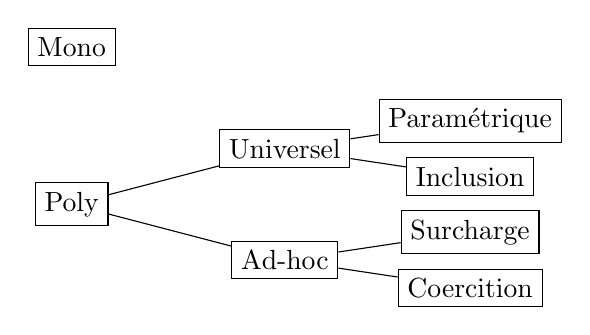
\begin{tikzpicture}
  [ ptype/.style={draw=black,shape=rectangle}
  , child/.style={ptype, xshift=2cm}
  , gen0/.style={       node distance=2cm}
  , gen1/.style={child, node distance=1cm}
  , gen2/.style={child, node distance=5mm}
  ]

  \node[ptype]                     (mono) {Mono};
  \node[ptype,below of=mono, gen0] (poly) {Poly};
  \node[above right of=poly, gen1] (univ)  {Universel};
  \node[above right of=univ, gen2] (param) {Paramétrique};
  \node[below right of=univ, gen2] (inclu) {Inclusion};
  \node[below right of=poly, gen1] (adho)  {Ad-hoc};
  \node[above right of=adho, gen2] (over)  {Surcharge};
  \node[below right of=adho, gen2] (coer)  {Coercition};

  \draw (poly) -- (univ);
  \draw (poly) -- (adho);

  \draw (univ) -- (param);
  \draw (univ) -- (inclu);

  \draw (adho) -- (over);
  \draw (adho) -- (coer);

      %node {Mono}
      %node {Poly}
          %node {Universal}
              %node {Param}
              %node {Inclusion}
          %node {Ad-Hoc}
              %node {Surcharge}
              %node {Coercition}

\end{tikzpicture}

\caption{Les différents types de polymorphisme.}
\label{fig:types-de-polymorphisme}
\end{figure}

\subsubsection{Monomorphisme}

Une première solution peut être de forcer des types concrets, c'est à dire
qu'une même fonction ne pourra s'appliquer qu'à un seul type de données.

Il est confortable pour le programmeur de n'avoir à écrire un algorithme qu'une
seule fois, indépendemment du type des éléments considérés.

\subsubsection{Polymorphisme universel}

% = {paramétrique, par inclusion}

\subsubsection{Polymorphisme ad-hoc}

% = {par surcharge, par coercition}

\subsubsection{Polymorphisme paramétrique}

Considérons la fonction de retournement de liste suivante :

\insertcode{listrev.ml}

Elle n'opère que sur la structure du type liste (en utilisant ses constructeurs
\texttt{{[}{]}} et \texttt{(::)} ainsi que le filtrage) : les éléments de
\texttt{lx} et \texttt{ly} ne sont pas manipulés à part pour les transférer dans
le résultat.

Moralement, cette fonction est donc indépendante du type de données contenu dans
la liste : elle pourra agir sur des listes de n'importe quel type d'élément.

Plutôt qu'un type, on peut lui donner un \emph{schéma de types} :

\[
  \textrm{append} : \forall a . a \textrm{list}
                             -> a \textrm{list}
                             -> a \textrm{list}
\]

Cela veut dire que \texttt{append} peut être utilisé avec n'importe quel type
concret \texttt{a} en \emph{instanciant} ce schéma de type (en substituant les
variables quantifiées par des types quelconques).

\subsubsection{Polymorphisme par inclusion}

\subsubsection{Polymorphisme par surcharge}

\subsubsection{Polymorphisme par coercition}


\subsection{Expressivité, garanties, types dépendants}

\section{Exemples}

\subsection{Faible dynamique : Perl}
\subsection{Faible statique : C}
\subsection{Fort dynamique : Python}
\subsection{Fort statique : OCaml}
\subsection{Fort statique à effets typés : Haskell}
\subsection{Theorem prover : Coq}
